



\section{DG for Possion Problem}%
\subsection{Possion Problem}%
\label{sub:possion_problem}

Lets define the problem \[
\begin{split}
    -\varepsilon \nabla u &= f \quad \text{in } \Omega   \\
    u&= u_{D} \quad \text{on } \Gamma _{D} \\
    \partial _{n} u & = g \quad \text{on } \Gamma _{N} \\
    \partial _{n} u +  \beta u & = h \quad \text{on } \Gamma _{R}
\end{split}
\]
Here is $\partial \Omega  = \Gamma _{D} \cup \Gamma _{N} \cup \Gamma _{R}$.

\subsection{Classical DG}%
\label{sub:classical_dg}

% \subsection{Apriori Error Analysis}%
% \label{sub:apriori_error_analysis}

% \subsection{Numerical Experiments}%
% \label{sub:apriori_error_analysis}



\subsection{Hybrid DG Method} %
\label{sec:hybrid_dg_method}

 We want to write this on a weak form. Let
the spaces we work on be \[
    \begin{split}
H^{1}\left( \mathcal{T}_{h}  \right) & = \left\{ u \in L^2\left( \Omega  \right), u \in H^{1 } \left( T \right) \forall T
\in  \mathcal{T} _{h }\right\} \\.
    \end{split}
\]

For the problem to be discontinuous do we define the trial and test function to be $u \in H^{1 }\left( \Omega  \right) $

and $v \in H^{1 } \left( \mathcal{T} _{h} \right)$. Thus,
\begin{equation}
\label{eq:1a}
- \sum_{T \in \mathcal{T} _{h}}^{} \int_{ T}^{}   \varepsilon \nabla ^2 u \cdot v dx = \sum_{T \in \mathcal{T}_{h} }^{}
\left\{ \int_{T}^{} \varepsilon \nabla u \nabla v dx - \int_{\partial T}^{} \varepsilon\cdot  \partial _{n} u \cdot v ds
\right\} = \sum_{T \in \mathcal{T} _{h}}^{}  \int_{T}^{} f\cdot v dx
.\end{equation}

But we want to introduce the shorter notation equivalently such that
\begin{equation}
\label{eq:1b}
   \sum_{T \in \mathcal{T} _{h}}^{}
     \left\{ \varepsilon\left( \nabla u, \nabla v \right) _{T} -\varepsilon \left<\partial _{n} u,v \right>_{\partial T} \right\} = \sum_{T \in
  \mathcal{T} _{h}}^{}  \left( f,v \right)
.\end{equation}

Where $\left< \cdot ,\cdot  \right>$ is the surface integral operator. Before we contitinue do we want to introduce a
alternative method to integrate using edges. Let $v_{F} \in  L^2\left( \mathcal{F}_{h}  \right)$ for the set of all
facets $\mathcal{F} _{h}$. Now the surface integral can be rewritten such that
\begin{equation}
\label{eq:2}
    \begin{split}
 \sum_{T \in
\mathcal{T} _{h}}^{} \varepsilon  \left<\partial _{n} u , v_{F} \right>
&= \sum_{E \in \mathcal{F} ^{int}}^{}  \varepsilon \left<\partial _{n^{+}} u, v_{F} \right>_{E} + \varepsilon \left<
\partial _{n^{-}} u, v_{F}
\right>_{E} + \sum_{E \in \mathcal{F} ^{ext}}^{} \varepsilon \left<\partial _{n} u, v_{F} \right>   \\
    \end{split}
.\end{equation}
Here are we using the definitions $n^{+}$ and $n^{-}$ illustrated using figure \ref{fig:normal_npluss}.
Lets define some crucial spaces for the DG method \[
    \begin{split}
V &=  \left\{ \left( u, u_{F} \right) : u \in H^2\left( \mathcal{T} _{h} \right) \cap H^{1}\left( \Omega  \right)   ,
u_{F} \in  L^2\left( \mathcal{F} _{h} \right)  \right\} \\
V_{h} &=  \left\{ \left( u,u_{F} \right) : u \in  \mathcal{P} ^{k} \left( T \right) \forall T \in  \mathcal{T} _{h} , \quad
u_{F} \in  \mathcal{P} ^{k}\left( E \right)  \forall E  \in \mathcal{F} _{h}   \right\} \\
    \end{split}
\]
\todo[inline]{ What is the intuition of a polynomial $\mathcal{P} ^{k} \left( E \right) $ along a edge? }
and now including drichlet conditions using the previous definition \[
\begin{split}
    V_{D} & = \left\{ \left( u,u_{F} \right) \in V , u_{F} = u_{D} \quad  \text{on } \Gamma _{D}  \right\} \quad
    V_{h,D}  = \left\{ \left( u, u_{F} \right) \in  V_{h}, u_{F} = u_{D} \quad  \text{on } \Gamma _{D}  \right\} \\
    V_{0} & = \left\{ \left( u,u_{F} \right) \in V , u_{F} = 0 \quad  \text{on } \Gamma _{D}  \right\} \quad
    V_{h,0}  = \left\{ \left( u, u_{F} \right) \in  V_{h}, u_{F} = 0 \quad  \text{on } \Gamma _{D}  \right\}
\end{split}
\]

Defining  $\left( u, u_{F} \right) \in  V_{D} $ and $\left( v, v_{F} \right) \in  V_{0} $.
Now adding \eqref{eq:1b} and \eqref{eq:2} can we easily see that
\begin{equation}
    \label{eq:3a}
    \begin{split}
   \sum_{T \in \mathcal{T} _{h}}^{}
     \left\{ \varepsilon\left( \nabla u, \nabla v \right) _{T}  \right\}
     & = \sum_{T \in \mathcal{T} _{h}}^{}  \left( f,v \right)_{T} +\sum_{E \in \mathcal{F} ^{int}}^{}  \varepsilon \left<\partial _{n^{+}} u, v_{F} \right>_{E} + \varepsilon \left<
\partial _{n^{-}} u, v_{F} \right>_{E} + \sum_{E \in \mathcal{F} ^{ext}}^{} \varepsilon \left<\partial _{n} u, v_{F} \right>
    \end{split}
.\end{equation}

\begin{figure}[!h]
\centering
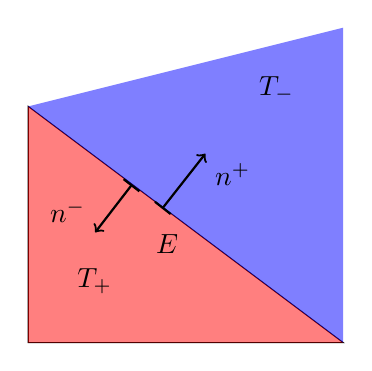
\begin{tikzpicture}[scale=1]
\coordinate (A) at (0,0);
\coordinate (C) at (0,3);
\coordinate (B) at (4,0);
\coordinate (D) at (4,4);
\coordinate (Tm) at (3.5,3.5);
\coordinate (Tp) at (0.5, 0.5);
\coordinate (e) at (1.5, 1.5);
\coordinate (start) at (1.7, 1.7);
\coordinate (end) at (2.25, 2.4);

\coordinate (start2) at (1.32, 2.01);
\coordinate (end2) at (0.85, 1.4);

\draw (A) -- (B) -- (C) -- cycle;
\fill[red, opacity=0.5] (A) -- (B) -- (C);
\fill[blue, opacity=0.5] (B) -- (C) -- (D);
\node[below left] at (Tm) {$T_{-} $ };
\node[above right] at (Tp) {$T_{+}$ };
\node[below right] at (e) {$E$ };

\draw [|->, thick] (start) -- (end);
\draw [|->, thick] (start2) -- (end2);
% \node[above right] at (A) {A };
% \node[below right] at (B) {B};
% \node[above right] at (C) {C };
% \node[below right] at (D) {D};
\node[below right] at (end) {$n^{+}$};
\node[above left] at (end2) {$n^{-}$};
\end{tikzpicture}
\caption{Edge $E$ shared by the triangles $T_{-}$ and $T_{+}$ and the normal unit vectors $n^{+}$ and $n^{-}$.  }
    \label{fig:normal_npluss}
\end{figure}


Applying the Neumann conditions on $ \Gamma _{N} $ and $\Gamma _{R}$, can the condition on the exterior facets
be rewritten such that
\[
\sum_{E \in \mathcal{F} ^{ext}}^{}  \varepsilon \left< \partial _{n} u, v_{F} \right> = \varepsilon \left<g,v_{F}
\right> _{\Gamma _{N}} + \varepsilon \left<h - \beta u, v_{F} \right> _{\Gamma _{R}}
\]
Keep in mind that we on the exterior boundaries define the integral so $\left<f, v_{F} \right>_{\Gamma } = \int_{\Gamma }^{} f
\cdot v_{F} \cdot n ds $ for a arbitary neumann boundary function $f$ on some surface $\Gamma $. Hence \eqref{eq:3a} ends up
being
\begin{equation}
\label{eq:3b}
 \sum_{T \in \mathcal{T}_{h} }^{} \varepsilon \left( \nabla u , \nabla v \right)  - \sum_{E \in F^{int}}^{} \left(
\varepsilon  \left<\partial _{n^{+}} u , v_{F} \right> _{E} + \varepsilon \left<\partial _{n^{-}}  u, v_{F}\right>_{E}
\right) +  \beta \left< \varepsilon  u, v_{F} \right> _{\Gamma _{R}} = \sum_{T \in T_{h}}^{} \left( f,v \right)_{T}   + \left<g, v_{F}
\right>_{\Gamma _{N}} + \left<h, v_{F} \right>_{\Gamma _{R}}
.\end{equation}

According to Lehrenfeld 2010  \cite{lehrenfeld2010} at page 13 on equation (1.2.7)  is \eqref{eq:3b} equivalent to

\begin{equation}
\label{eq:3c}
\sum_{T \in \mathcal{T} _{h}}^{}   \left( \varepsilon \nabla u, \nabla v \right) _{T} -\sum_{T \in \mathcal{T} _{h}}^{}    \left<\varepsilon  \partial
_{n} u , \jump{ v } \right> _{\partial T}  + \beta  \left< \varepsilon u, v_{F}  \right>_{\Gamma _{R}} = \sum_{T
\in \mathcal{T} _{h}}^{} \left( f,v \right)  + \left<\varepsilon g, v_{F} \right>_{\Gamma _{N}} + \left<\varepsilon h,
v_{F} \right>_{\Gamma _{R}}
\end{equation}

Where, $u, u_{F} \in V_{D}$ and $v, v_{F} \in V_{h}$
Here is the jump defined simply as $\jump{v} = v - v_{F}$. Remember that $ v_{F} = tr_{\partial T} \left( v \right)  $. What we see is for \eqref{eq:3b} and \eqref{eq:3c} to be
equivalent must this be true.
\begin{equation}
\label{eq:3c4}
    \sum_{T \in \mathcal{T} _{h}}^{}  \left< \varepsilon \partial _{n} u, \jump{v}  \right>_{\partial T} = \sum_{T \in
    \mathcal{T} _{h}}^{}  \left< \varepsilon \partial _{n} u, v  \right>_{\partial T} - \left< \varepsilon
    \partial _{n} u, v_{F}  \right>_{\partial T} =\sum_{E \in
    \mathcal{F} ^{int}}^{}  \varepsilon \left( \left< \partial _{n^{+}} u, v_{F} \right>_{E}  + \left<\partial _{n^{-}}
u, v_{F}\right> \right)
.\end{equation}

\todo[inline]{why is it true?}


Since $\left( u, u_{F} \right) \in V $ is has to be continious, hence the jump is $\jump{u} = 0$ for the correct
solution. Hence,
adding $-\left<\varepsilon \partial _{n} v, \jump{u} \right>_{\partial T}$ for symmetry and $ \tau _{h} \left<\varepsilon \jump{u},
\jump{v} \right>_{\partial T}$ for stability with some stabilization parameter $\tau _{h}$ for each $T \in
\mathcal{T}_{h} $. This can be added to lhs on \eqref{eq:3c} such that,

\begin{equation}
\label{eq:3c3}
\begin{split}
    \sum_{T \in \mathcal{T} _{h}}^{}   \left( \varepsilon \nabla u, \nabla v \right) _{t} &-\sum_{T \in \mathcal{T} _{h}}^{}
\left\{ \left<\varepsilon  \partial
_{n} u , \jump{ v } \right> _{\partial T}  -\left<\varepsilon
\partial _{n} v, \jump{u} \right>_{\partial T}  + \tau _{h} \left<\varepsilon \jump{u},
\jump{v} \right>_{\partial T} \right\}  \\ &+ \beta  \left< \varepsilon u, v_{f}  \right>_{\Gamma _{R}} \\
                                           &= \sum_{T
\in \mathcal{T} _{h}}^{} \left( f,v \right)  + \left<\varepsilon g, v_{F} \right>_{\Gamma _{N}} + \left<\varepsilon h,
v_{F} \right>_{\Gamma _{R}}
\end{split}
\end{equation}



Finally, we can now construct the discrete system. Let now $u, u_{F} \in V_{h,D}$ and $v, v_{F} \in V_{h,0}$ be the
discretized spaces. Using what we have in \eqref{eq:3c} can we define \[
    \begin{split}
F\left( v, v_{F} \right) & =  \sum_{T
\in \mathcal{T} _{h}}^{} \left( f,v \right)  + \left<\varepsilon g, v_{F} \right>_{\Gamma _{N}} + \left<\varepsilon h,
v_{F} \right>_{\Gamma _{R}} \\
B\left( u, u_{F} , v, v_{F} \right)  &=
    \sum_{T \in \mathcal{T} _{h}}^{}   \left( \varepsilon \nabla u, \nabla v \right) _{t} -\sum_{T \in \mathcal{T} _{h}}^{}
\left\{ \left<\varepsilon  \partial
_{n} u , \jump{ v } \right> _{\partial T}  -\left<\varepsilon
\partial _{n} \jump{u} \right>_{\partial T}  + \tau _{h} \left<\varepsilon \jump{u},
\jump{v} \right>_{\partial T} \right\}  + \beta  \left< \varepsilon u, v_{F}  \right>_{\Gamma _{R}} \\
    \end{split}
\]

\begin{equation}
\label{eq:3f }
B\left( u, u_{F} , v, v_{F} \right) = F\left( v, v_{F} \right)
.\end{equation}






z
